\documentclass[10pt,a4paper]{report}

\usepackage[utf8]{inputenc}
\usepackage[francais]{babel}
%\usepackage[english]{isodate}
\usepackage[parfill]{parskip}
% pour les images
\usepackage{graphicx}
% pour les images eps
\usepackage{epstopdf}
% pour la coloration syntaxique
\usepackage{listings}
% pour xml
\usepackage{color}
\definecolor{gray}{rgb}{0.4,0.4,0.4}
\definecolor{darkblue}{rgb}{0.0,0.0,0.6}
\definecolor{cyan}{rgb}{0.0,0.6,0.6}
\lstset{
  basicstyle=\ttfamily,
  columns=fullflexible,
  showstringspaces=false,
  commentstyle=\color{gray}\upshape
}
\lstdefinelanguage{XML}
{
  morestring=[b]",
  morestring=[s]{>}{<},
  morecomment=[s]{<?}{?>},
  stringstyle=\color{black},
  identifierstyle=\color{darkblue},
  keywordstyle=\color{cyan},
  morekeywords={xmlns,version,type}% list your attributes here
}

\title{Rapport de projet de BDASIM\\Système d'Information et XML - Base de données fédérée}
\author{
	Bastien Berge \\
	Alban Granger \\
	Léo Guirinec \\
	Richard Lagrange \\
	Chunli Li \\
	Brendan Masson \\
	Martin Seillan \\
}
%\date{''date de fin de rédaction''} 

\begin{document} 
\maketitle

\pagenumbering{Roman}
\tableofcontents
\newpage
\listoffigures
\newpage
\listoftables
\newpage
\pagenumbering{arabic}
\lstset{ %
  backgroundcolor=\color{white},   % choose the background color; you must add \usepackage{color} or \usepackage{xcolor}
  basicstyle=\footnotesize,        % the size of the fonts that are used for the code
  breakatwhitespace=false,         % sets if automatic breaks should only happen at whitespace
  breaklines=true,                 % sets automatic line breaking
  captionpos=b,                    % sets the caption-position to bottom
  deletekeywords={...},            % if you want to delete keywords from the given language
  escapeinside={\%*}{*)},          % if you want to add LaTeX within your code
  extendedchars=true,              % lets you use non-ASCII characters; for 8-bits encodings only, does not work with UTF-8
  frame=single,                    % adds a frame around the code
  keepspaces=true,                 % keeps spaces in text, useful for keeping indentation of code (possibly needs columns=flexible)
  keywordstyle=\color{blue},       % keyword style
  language=SQL,                 % the language of the code
  morekeywords={*,...},            % if you want to add more keywords to the set
  numbers=left,                    % where to put the line-numbers; possible values are (none, left, right)
  numbersep=5pt,                   % how far the line-numbers are from the code
  rulecolor=\color{black},         % if not set, the frame-color may be changed on line-breaks within not-black text (e.g. comments (green here))
  showspaces=false,                % show spaces everywhere adding particular underscores; it overrides 'showstringspaces'
  showstringspaces=false,          % underline spaces within strings only
  showtabs=false,                  % show tabs within strings adding particular underscores
  stepnumber=2,                    % the step between two line-numbers. If it's 1, each line will be numbered
  tabsize=2,                       % sets default tabsize to 2 spaces
  title=\lstname                   % show the filename of files included with \lstinputlisting; also try caption instead of title
}

\graphicspath{{ressources/graphiques}}
 
\chapter*{Introduction}
\addcontentsline{toc}{chapter}{Introduction}
De nos jours, la plupart des entreprises peuvent être vues comme un ensemble de services, traitant des données hétérogènes en utilisant des technologies variées. De plus, ces mêmes données peuvent être stockées de manières différentes, via par exemple des bases de données relationnelles ou graphes, des fichiers XML, etc. L’un des rôles du système d’information est donc de structurer et gérer ces données. Cependant l’accès à ces données peut poser des difficultés. En effet, il est impensable de comparer ou de joindre des données issues de  sources différentes. Ce problème est pourtant inévitable puisque le contexte des systèmes d’informations modernes implique souvent des systèmes de gestion de bases de données différents au sein d’une même entreprise.

Pour pallier à cela, des architectures de bases de données permettent d'accéder à des données de nature complètement différente. Parmi ces architectures, les principales sont les bases de données fédérées et les “data warehouses” (entrepôts de données). Dans le cadre du projet de Bases de Données Avancées et Systèmes d’Information Modernes, nous étudierons le système de bases de données fédérée et nous mettrons en oeuvre une fédération de divers bases de données, telles qu’une base de données relationnelles et une base de données XML. Le but de ce travail est d'identifier les différentes étapes et modules qui entrent en jeu lorsqu'une requête est effectuée sur une base de données fédérée. Afin de comprendre les différents problèmes inhérents à la fédération, nous avons décidé de réaliser une telle base qui devra pouvoir traiter une requête, de l'émission de la requête par le client jusqu'à la production d'une réponse fédérée, en passant par le traitement dans chaque base. Cette requête se voudra simplifiée afin de pouvoir aborder tous les aspects possibles dans le court temps imparti.

\chapter{Présentation des bases de données fédérées}
\section{Présentation des bases de données fédérées}

\subsection{Idée générale}

Les bases de données fédérées ont pour but de proposer une vue unique à un ensemble de bases de données de diverses natures. Ces bases de données peuvent être séparées géographiquement. L’utilisateur consulte ainsi les données soumises un modèle unifié et cohérent.

Cette problématique intervient particulièrement lors de la fusion de systèmes d’information, voire d’entreprises, lorsqu’on souhaite associer des bases de données différentes sans pour autant les regrouper dans une base unique et homogène, ce qui aurait un coût très important.

L’accès aux données et leurs mises à jour se font via un langage unique, ce qui donne une certaine transparence, puisque l’utilisateur ne se préoccupe pas de savoir dans quelles bases se trouvent les données qu’il souhaite et quel est le langage à appliquer pour les récupérer.

La base de données fédérée se doit aussi d’être extensible, afin de permettre l’intégration de nouvelles bases, possiblement utilisant encore une technologie différente. De plus, chaque base est rendue autonome, ce qui va dans le sens de l’extensibilité. Enfin, la base de données fédérées est avant tout une base de données, et doit remplir son rôle en gardant en tête les contraintes de performances, aspect important des bases de données.

Pour finir, gardons à l’esprit l’existence possible de conflits, de par la nature même des bases de données fédérées. Ces conflits, directement liés à l’hétérogénéité des différentes bases fédérées, se doivent d’être identifiés et gérés lors de la procédure de fédération. C’est aussi ce genre de difficulté que ce projet nous permettra d’appréhender plus facilement à l’avenir.


\subsection{Fonctionnement avec une requête simple}

Afin d’appréhender le fonctionnement général d’une base de données fédérée, étudions le parcours d’une requête simple. Cette requête est émise par l’utilisateur en XQuery et prend la forme suivante :

\begin{verbatim}
for $nom in doc()//nom

where $nom/..//age > 18

return $nom
\end{verbatim}

Supposons la base de données fédérée comme composée de deux bases : l’une qu’on appellera R1 est une base de données SQL et contient deux colonnes “id” et “nom”, l’autre appelée R2 est une base de données XML et contient des “personnes” possédant un élément “id” et un élément “age”. 

\begin{figure}[h!]
    \centering
    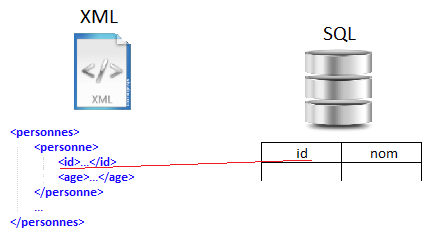
\includegraphics[width=0.8\textwidth]{ressources/graphiques/xmlAndSql_simple_example.png}
    \caption{Exemple simplifié d'une base fédéré}
\end{figure}


Avec cette requête, l’utilisateur cherche à accéder au nom des personnes présentes dans la base fédérée étant majeures. Elle est effectuée en accord avec un schéma fédéré, qui est défini pour représenter la structure virtuelle de la base de données vue par l’utilisateur.

La requête est transmise au médiateur, élément central de l’architecture fédérée. Pour commencer, le médiateur fait vérifier l’intégrité et le bon format de cette requête par le module verifier. Si ce module n’accepte pas la requête, elle est abandonnée. Sinon, il va diviser la requête, via son module splitter dans le but d’adresser les sous-requêtes aux bonnes bases de données. Dans notre cas, on aura une sous-requête sur R2 demandant la liste des “id” dont “age” est supérieur à 18, et une sous-requête sur R1 qui rendra la liste des “noms” dont les “id” ont été rendus par la première sous-requête. Mais avant d’être émises, ces sous-requêtes seront traduites dans un langage pivot.

Ces sous-requêtes traduites sont transmises aux différents wrappers chargés de chaque base de données concernée. Le wrapper W2 reçoit la requête qui concernera R2 et la traduit donc en XQuery afin d’interroger R2. Il capte ensuite la réponse de R2, la traduit et l’envoie au médiateur. De même W1 traduira, cette fois-ci en SQL, et transmettra la réponse traduite au médiateur.

C’est cette fois-ci le module merger du médiateur qui entre en jeu et remplit son rôle de fusion des réponses des différentes sous-requêtes dans le but de répondre à la requête initiale.

Enfin, un helper pourra intervenir en sortie du médiateur pour traduire la réponse dans le langage souhaité.

\subsection{Les bases de données fédérées}

\subsubsection{Couplage de bases de données}

Il existe deux grands types de bases de données fédérées : les bases faiblement couplées et les bases fortement couplées. Nous nous sommes intéressés pour ce projet aux bases de données fédérées faiblement couplées

En effet, les bases fortement couplées sont constituées d’un ensemble de bases ayant accès à toutes les autres bases. Chaque base fédérée est chargée de s’occuper de l’interfaçage avec les autres bases. Pour N base fédérées, chaque base doit implémentées N - 1 interfaces, ce qui représente au total N(N-1)/2 interfaces au totales. Nous avons donc choisi d’étudier l’autre modèle qui apporte plus de flexibilité. Dans la suite nous traiterons uniquement du cas faiblement couplé.

L’idée générale de ce modèle est de regrouper sous un modèle unique des bases de données hétérogènes. L’architecture est consituée de couches d’abstraction successives. Les données qui passent à travers les couches sont transformées de manière à découpler la représentation des données de leur stockage physique.

Les données sont transmises à travers un certain nombre de couches. Ces couches communiquent entre elles grâce à un langage intermédiaire de haut niveau. Chaque couche possède une représentation des données de la base qui lui sont propres, et est constituée de composants appellés “wrappers”. La couche la plus basse se charge de l’interfaçage des sources avec la fédération.

Nous utilisons des schémas pour qualifier ces représentations des données propres à chaque couches. Nous utilisons quatre niveaux dans notre étude :

\begin{itemize}
    \item Le schéma externe : la représentation des données manipulée par l’utilisateur ;

    \item Le schéma fédéré : la représentation interne des données agrégées ;

    \item Le schéma composant : la représentation des données communiquée aux sources ;

    \item Le schéma local : la représentation des données dans les sources.
\end{itemize}

\subsubsection{Problèmes communs liés aux architectures fédérées}

La fédération de sources différentes ou distantes pose naturellement des difficultés récurrentes. A partir de l’ouvrage Database Systems, nous avons cherché à étudier et appréhender les problèmes liés à l’architecture fédérée. Ces problèmes peuvent provenir directement des situations suivantes :

\begin{itemize}
    \item hétérogénéité de la communication : différents systèmes reposent généralement sur différents protocoles de communication et ces différents protocoles sont à traiter indépendemment les uns des autres ;
    \item hétérogénéité des langages de requête : différents systèmes emploient différents langages de requêtes, ces langages sont en particulier variable selon le type des bases considérées, par exemple XQuery pour XML ou Cypher pour Neo4j ;
    \item hétérogénéité des schémas : différents types de données peuvent être représentés de manières différentes, par exemple un objet comportant d’autres sous-objets pourra être représenté par des balises internes en XML et par des références vers des tables (clefs étrangères) en SQL ;
    \item  hétérogénéité des types : des données peuvent parfois être représentées par des types différents selon l’implémentation, par exemple un numéro de téléphone peut être vu comme un entier ou une chaîne de caractères ;
    \item hétérogénéité sémantique : certaines données peuvent être regroupées dans différentes catégories sémantiques, exemple une première base peut considérer un personnage comme un “adjuvant” ou une autre comme un “humain”.
\end{itemize}

Cependant, ces problèmes sont généralement traités par l’architecture même de la fédération. En effet, on pourra résoudre les problèmes liés à l’hétérogénéité de communication ou de langages de requêtes grâce à point d’accès unique vers la base. L’hétérogénéité des schémas est masquée par des étapes successives de transformation et la représentation interne. Enfin, l’hétérogénéité des types peut être gommée dans les couches basses de la fédération, notamment par l’action des wrappers.




\chapter{Présentation du projet}
\section{Présentation du projet}

\subsection{Présentation de notre modèle}

\subsubsection{Les différentes bases}

Pour notre projet, nous avons décidé de fédérer deux bases de données hétérogènes : une base de données relationnelles et une base de données XML. Les données présentes dans ces bases modélisent des pokémons. Les pokémons sont des monstres issus de la culture japonaise. Ces pokémons possèdent un ou plusieurs types (feu, eau, plante…) et des compétences. Ils sont possédés par des dresseurs. Ces dresseurs forment des équipes. Une description plus complète de ce contexte est faite en annexe A.

La base SQL possède une table synthétisant certaines des caractéristiques des pokémons.
\begin{itemize}
\item id : identifiant du pokémon	
\item name : nom du pokémon	
\item height, weight : taille et poids du pokémon	
\item base\_experience : base servant à calculer, après application de coefficients, le gain réel d’expérience
\end{itemize}

\begin{tabular}{|c|c|c|c|c|}
 \hline
 id & name & height & weight & base_experience \\
 \hline
\end{tabular}

La seconde base de données, la base XML, dispose de 3 fichiers XML : pokémons.xml, teams.xml et moves.xml. Le fichier pokémons.xml regroupe le ou les types de chaque pokémon. Le fichier teams.xml regroupe toutes les teams. Une team est composée d’un dresseur de pokémons. Ce fichier permet de savoir quels pokémons possédait chaque team. Enfin le fichier moves.xml regroupe tous les moves existants, c’est-à-dire toutes les compétences que peuvent avoir les pokémons.


 \subsubsection{Schéma externe}

Du point de vue de l’utilisateur, les données issues des différentes bases sont regroupées sous un même modèle appelé schéma externe. Lorsque le client veut accéder à des données, il effectue une requête sur ce modèle. La réponse qu’il obtiendra respectera également le modèle du schéma externe.

Le schéma externe est représenté par le fichier xsd présent en Annexe B.

\subsection{Implémentation de la base de données fédérée}

Pour implémenter notre projet, nous avons choisi d’utiliser le langage de script Python version 3.3 car ce dernier offre une grande flexibilité grâce à diverses librairies et une grande simplicité de code. Les principales librairies utilisées pour notre projet sont :

\begin{itemize}
    \item zorba : processeur qui permet d’effectuer des requêtes XQuery ;

    \item sqlite3 : librairie qui permet de faire des requêtes SQL sur une base SQLite ;

    \item xml.eTree : permet la manipulation de fichier XML et d’objet XML en Python (création, édition, etc.).
\end{itemize}

Chaque fonctionnalité est codée dans un fichier portant le nom de la fonctionnalité implémentée.

/* Schéma avec les fichiers et les appels aux autres fichiers */

Le schéma est dans le drive : à inclure OK

/* Détails expliqué “tel script a tel rôle et appelle tel script…”*/

Le client, souhaitant interroger son système d’information, lance une requête XQuery. Cette requête ne prend pas en compte la totalité de la syntaxe XQuery mais une limitation assez basique de cette dernière : l’utilisateur peut uniquement effectuer des “for … where … return …” et les requêtes imbriquées ne sont pas gérées. De plus les conditions sont triviales avec toujours un couple variable/valeur (par exemple, where $var <> “valeur”). Pour ce qui est du return, il renverra tout le temps la variable définie dans le for.

\subsubsection{Verifier}

La requête passe en premier lieu par le “Verifier”. Ce dernier a pour rôle de contrôler la requête, c’est-à-dire vérifier la syntaxe. Cette vérification est autant lexicale, que syntaxique, puisqu’il s’agit notamment de vérifier que la requête se limite bien à la syntaxe proposée. La vérification possède également un aspect sémantique, et en particulier, le “Verifier” certifie que les noms des tables utilisés sont reconnus. Si le “Verifier” valide la requête, cette dernière est envoyée au “Splitter”.

\subsubsection{Splitter}

Le “Splitter” doit séparer la requête en autant de sous-requêtes qu’il faut faire dans les sous-bases (sous-requête = lecture d'une table SQL ou un fichier XML).faut consulter de fichiers XML et de tables SQL. Par exemple si la requête initiale concerne un fichier XML et deux tables SQL, malgré la présence d’une unique base de données SQL pour deux tables, trois sous-requêtes seront crées.

Prenons l’exemple suivant de requête XQuery :

for \$type in doc()//team[victory > 10]/pokemon/type1

where \$type <> “Grass”

return \$type

La partie for sera analysée et divisée selon son contenu. On se concentre seulement sur la partie xPath de l’expression :

//team[victory > 10]/pokemon/type1

On lui ajoute ensuite la condition de son where en syntaxe xpath en faisant attention à sa position relativement dans le schéma fédéré.

//team[victory > 10]/pokemon/type1[. <> “Grass”]

On découpe ensuite notre requête en ne gardant que les attributs non virtuels (attributs réellement présents dans une des sous-bases) :


[victory > 10]


[. <> “Grass”]


type1 (valeur de retour, dernier attribut de la clause for)

On analyse ensuite séquentiellement de haut en bas. Toutes ces lignes seront comparées à la dernière (type1), puisque ce sera le résultat rendu. On simule le fait de partir avec l’ensemble des type1 existants. Ensuite, on filtre cette ensemble avec les conditions (victory > 10) et (type <> “Grass”). On obtiendra ainsi l’ensemble des résultats type1 bien filtrés.



Pour corréler type1 avec victory, on utilise un algorithme de décision.

Partie du schéma fédéré qui nous intéresse dans cet exemple :

Légende (losange : attribut virtuel, rond : attribut réel, note : cluster où trouver l’attribut)

Dans la première étape, il nous faut relier victory et type1. On utilise un algorithme de décision qui nous donnera la jointure à faire pour relier deux “clusters” (cluster = une table de base ou un fichier xml /* en footnote */). Ici on relie C4 et C1. L’algorithme nous donnera la démarche à suivre pour tout relier.

C1 --id1→ C2 --id2→  C4

En supposant que ces clusters soient tous dans des bases SQL, on fait les deux sous-requêtes suivantes pour joindre victory et type1 :

SELECT id1 FROM C1 WHERE victory > 10

SELECT id2 FROM C2 WHERE id2 = id1


Il se peut que ces sous-requêtes aient besoin d’interroger plusieurs tables ou fichiers, et soient aussi une requête de bases de données fédérées. Tant qu’elles interrogent plusieurs tables ou fichiers, elles sont sous-divisées jusqu’à devenir simples. La complexité de la requête est réduite (on obtient une sous-requête moins compliquée que la précédente), et donc en procédant de façon récursive, on arrivera à répondre aux requêtes éventuellement.

Une fois la sous-requête prête, elle sont envoyées pour interroger les bases. Des objets sont retournés. Ces objets, pas forcément utiles aux données demandées dans la requête principale, sont réceptionnés, et sont transformés en tant que conditions supplémentaires de la requête principale.

L’attribut intéressant pour réaliser la sélection est extrait. E.g. : les id2 sont récupérés afin de restreindre type1.

id2 nous a retourné 5 et 6., on produit donc :

selection = “id2 = 5 or id2 = 6”

Ensuite, on analyse [. <> “Grass”]. On le simplifie immédiatement puisqu’il s’agit exactement de l’attribut de retour. L’ultime variable selection est mise à jour:

selection = “id2 = 5 or id2 = 6 or type <> ‘Grass’”

La requête ultime qui renverra le résultat escompté sera tout simplement :

“SELECT type1 FROM C4 WHERE “ + selection

Soit :

SELECT type1 FROM C4 WHERE id2 = 5 or id2 = 6 or type <> ‘Grass’

En conclusion, grâce à l’arbre représentant le schéma fédéré, nous arrivons a recréer une requete plus simple, touchant à une unique table,  sans avoir à effectuer de joins, la sélection ayant eu lieu plus tôt grâce aux sous-requêtes.

\subsubsection{Wrapper}

Les sous-requêtes sont exprimées dans un langage pivot, compréhensible par tous les “Wrapper” (voir 3) b) ). Les sous-requêtes sont poussées vers les “Wrapper”.

Ces derniers reçoivent la requête en langage pivot et commencent par la traduire vers un langage de requête propre à la base, requête SQL pour l’un et requête XQuery pour l’autre. Ils exécutent ensuite la requête auprès de la source de données. Le résultat ainsi produit est ensuite retransformé vers du XML, le langage de retour des “Wrapper”. Dans notre cas, l’un des wrappers éxecutant du XQuery, cette transformation est inutile car le résultat est déjà en XML, pour SQL, cependant, cette transformation a bien lieu. Le XML ainsi produit est retourné au “Mediator”.

C’est le “Merger” qui continue le traitement de la requête au sein du “Mediator”. La particularité des “Wrapper” est d’envoyer au “Merger” le même type de données. Cependant des informations peuvent correspondre au sein de ses données. Le rôle du “Merger” est de traiter ces données apparemment hétérogènes et d’en effectuer les liaisons, lorsque cela est judicieux. Dans notre modèle de données par exemple, les informations propres à une espèce de pokémon sont séparées et se trouvent à la fois dans un fichier XML (ses types) et dans une table SQL (son poids, sa taille, etc.). Lorsque l’utilisateur veut des données générales sur un pokémon donné (donc un “id” donné), le “Merger” devra ici joindre les deux parties de l’information par rapport à l’id. 

\subsection{Architecture et adaptations}

Dans le cadre de notre projet, nous avons décidé d’implémenter une chaîne simple. Les fonctionnalités de chaque niveau (source, médiator et client) sont simplifiées. En effet, il semble plus intéressant de créer une vue d’ensemble pour mieux appréhender une architecture telle que la fédération de bases de données. Ainsi notre application reposera sur la gestion de requêtes simples telle que l’interrogation des bases avec des conditions. En revanche, les mises à jour de bases ne sont pas implémentées car cela augmente grandement la complexité de l’architecture.

\subsubsection{L’architecture globale}

**** Insérer schéma UML (class_diagram.eps)****

Présenter l’architecture à l’aide du schéma, et souligner les différences par rapport à ce qui a été présenté dans I.

\subsubsection{Le langage pivot}

Comme évoqué plus haut, le “Splitter” exprime les sous-requêtes, à partir de la requête initiale, dans un langage pivot, que tous les “Wrapper” pourront comprendre et traduire en langage source. Ce langage pivot prend la forme d’un objet python, nommé Req. Cet objet correspond au découpage simple d’une requête en 3 éléments :

    - le nom des “colonnes” de projection ;

    - la partie sélection ;

    - le nom de la table/fichier XML.


Un objet Req pourra être instancié de la façon suivante :

Req( [ “name”, “description” ], “@id = 99”, "pokemon" ) // A mettre en code !

/* ** Pour inclure du code et lui donner de la couleur

http://en.wikibooks.org/wiki/LaTeX/Source_Code_Listings

*/

C’est donc cet objet qui sera transmis au bon “Wrapper”, et qui sera traduit en requête pour la source associée.

Notons que dans le cadre de ce projet, cet objet a été allégé au mieux : il interroge une seule table/un fichier xml de manière simple, à travers une projection, et une sélection. Cette sélection a été limitée à une combinaison, via des AND et des OR, de conditions dont le membre droit est une valeur non-variable. Ainsi, tous les problèmes liés à la fédération, de jointure par exemple, seront traités par le “Mediator”, en amont ou en aval.

\subsection{Modules et fichiers}

Présenter les modules/fichiers 1 par 1 en expliquant rapidement leurs interactions (si possible avec des références à 2)).

\subsubsection{“models.py”}

Ce fichier décrit le schéma fédéré, via la fonction schema(), et deux des classes majeures du programme : Req et Cluster. La classe Req décrit l’objet de requête envoyé aux différents aux wrappers et la classe Cluster représente un ensemble “table/fichier” et “wrapper” qui correspond à un objet interrogé.

\subsubsection{“fdb.py”}

Ce fichier est le fichier “main” et est en ce sens le point d’entrée du système.

\subsubsection{“fdb.py”}

Ce fichier comporte une fonction merge qui réalise la “jointure” entre les résultats des sous-requêtes. Cette fonction attend en paramètre un fichier xml qui est lui-même une concaténation des deux fichiers xml à joindre, un XSLT, qui est le XSLT effectuant le merge et le résultat sera stocké dans le troisième paramètre.

\chapter{Améliorations envisagées}
Nous allons maintenant présenter les différentes améliorations à apporter à notre architecture. En effet, notre projet ayant un intérêt d’abord pédagogique, nous avons simplifié plusieurs aspects. Cette partie liste et décrit les possibles pistes d’améliorations.

\section{Extension du langage de requête}

Comme nous l’avons expliqué, notre langage permet tout simplement de faire des accès aux bases avec des possibles conditions. Ce langage est donc assez basique. La première piste d’améliorations serait d’étendre le langage pivot. En plus de pouvoir consulter la base, l’utilisateur pourra faire des mises à jour et ordonner les résultats de ses requêtes. Ces fonctionnalités sont primordiales pour une système d’informations.

\section{Extension de la fédération}

Bien que notre projet ne comportait que deux sources de stockages, il est tout à fait possible d’ajouter de nouvelles sources comme des bases de données graphes, des fichiers CSV, etc. Cela aura comme effet d’augmenter le nombre de wrappers qui seront propres à chaque nouvelle source. Le schéma fédéré sera également plus important car les nouvelles sources impliqueront de nouvelles données.

\section{ Mise en cache des requêtes fréquentes}

Il serait avantageux de pouvoir mettre en cache les résultats des requêtes les plus fréquentes à tous les niveaux de l’architecture pour gagner en vitesse. Puisque les différents niveaux communiquent entre eux avec XML et XQuery, ils peuvent indépendemment mettre en cache des données ce qui éviterait de solliciter les sources et éviter des entrées-sorties. Ceci aurait pour potentielle conséquence négative des problèmes d’incohérences de données, par exemple si des mises à jour ont lieu et que les données mises en cache n’ont pas été mises à jour contemporainement. Cette proposition est donc à préférer pour des données peu fréquemment modifiées. Dans notre exemple cela pourrait s’appliquer aux fichiers “moves.xml”, “pokemon.xml” et à la table “pokemon”, en effet, ces données sont plus de l’ordre des métadonnées que de réelles données et sont très peu soumises à des mises à jour.

\section{Parallélisation et découplage}

L’architecture actuelle souffre de goulets d’étranglements au niveau des entrées-sorties. Nous gagnerions grandement en vitesse d’exécution si les différentes parties étaient parallélisées. Il serait possible de traiter les requêtes en flux tendu en implémentant des systèmes de producteurs/consommateurs ce qui permettrait d’obtenir des résultats avant que la requête n’ait  fini. Cela aura pour autre avantage d’alléger la taille en mémoire de l'application à un instant donné puisque chaque partie stockerait uniquement ce dont elle a besoin pour travailler.

\section{Jointures croisées déléguées aux sources}

Dans l’architecture actuelle, les jointures qui s’effectuent entre différentes sources sont calculées à l’intérieur même du médiateur. Cela engendre de nombreux aller-retours entre ces sources. Une gestion plus judicieuse serait de transformer les requêtes de telle sorte à déléguer au maximum les tâches de jointure aux sources pour profiter des avantages de la localité des données.

\chapter{Apports du projet}
Ce projet constitue une première expérience enrichissante dans le domaine des bases de données fédérées. Ce domaine est largement répandu dans le milieu des entreprises, puisque les bases de données se font de jour en jour à la fois plus variées et plus nombreuses. Cela nous a donc permis de nous familiariser à la mise en place d’une fédération de plusieurs bases de données différentes, en l’occurrence une base SQL et des fichiers XML.

La vastitude du sujet, et le court temps disponible à sa réalisation nous ont amenés à faire des choix, notamment en simplifiant et évitant en pratique différents problèmes liés à cette fédération. Cela nous a permis d’obtenir une vue globale de ce qu’est la fédération de bases de données. Pour autant, nous n’avons pas pour autant mis de côté l’aspect des conflits et difficultés liés à l’hétérogénéité de la base fédérée, et que nous avons décrit plus tôt. Nous avons donc acquis une connaissance générale des bases de données fédérées et des difficultés qui leur sont associées.

Malgré le temps imparti, et les conflits et difficultés de la fédération qui ont fait l’objet d’une autre partie de ce rapport, nous avons tenu à relever certains aspects et obstacles notables rencontrés lors du développement des différents modules du système fédéré.

\section{Verifier}

En entrée du système fédéré, nous avons besoin de contrôler les requêtes XQuery de l’utilisateur pour éviter toute erreur dans l’application. Cependant, il n’existe pas d’outil immédiat pour vérifier la validité d’une requête XQuery au niveau de ses chemins XPath.

Nous avons pu contourner le problème en convertissant les chemins dans les documents en chemins dans des schémas XSD. Ainsi, il est alors possible de vérifier la validité de ces chemins grâce à ces schémas.

\section{Splitter}

L’une des difficultés majeures rencontrées lors du développement du splitter a été le traitement des clauses where et la création de l’objet Req. Comme précisé en amont, nous avons sous-diviseés les requêtes en un objet python, Req, que nous voulions le plus simple possible. L’un des principaux avantages de cet objet est qu’il facilite la création des wrappers, le principal problème résultant est qu’il complique le travail du splitter, à qui revient la charge importante de bien discerner les sous-requêtes. Trouver la bonne représentation pour cet objet n’a pas été aisé et la classe Req est passée par différents états avant d’arriver à une solution satisfaisante. L’objet finale est composé d’un tableau regroupant les “colonnes” de la projection, d’une chaîne de caractère représentant la sélection et d’un nom de la table, ou du fichier, considéré. Ces éléments représentent des points communs à toutes les requêtes et pour tous nos types de bases de données. Cet objet se veut le plus généraliste possible pour ne pas être redesigné à chaque ajout d’une nouvelle source de données, par exemple des fichiers Excel.

\section{Merger}

Le rôle du merger est, comme expliqué plus tôt, de joindre les différentes réponses obtenues auprès de chaque source, afin de répondre correctement à la requête initiale. Chaque réponse aux sous-requêtes étant donnée en XML, il nous faut donc, au sein du Merger, joindre ces réponses XML en une seule.

Cependant, les deux premières solutions que se sont présentés à nous, à savoir la bibliothèque python lxml2 et les ElementTree de python, se sont révélées infructueuses, ou difficiles à mettre en place.

Afin de répondre à ce problème, nous avons utilisé XSLT. En pratique, le fichier xslt est appliqué aux deux fichiers à fusionner. Il trouve ainsi toutes les balises de chaque fichier, et les fusionne au besoin en fonction des attributs de ces balises. Seront donc considérées fusionnables les balises ayant un attribut commun et la valeur de cet attribut identique.



%\chapter*{Annexes} 
%\addcontentsline{toc}{chapter}{Annexes}
\appendix
%\addtocontents{toc}{\protect\setChapterprefix{Appendix }}
\paragraph{A - Extraits du modèle de données}
\hspace{0pt}

\lstinputlisting[language=SQL, firstline=1, lastline=10, caption={Extrait des requêtes de création de la table "pokemon"}]{ressources/textuelles/request_pokemon.sql}
\emph{(...)}
\lstinputlisting[language=SQL, firstline=724, lastline=726]{ressources/textuelles/request_pokemon.sql}

\lstinputlisting[language=SQL, firstline=1, lastline=10, caption={Extrait des requêtes de création de la table "team"}]{ressources/textuelles/request_team.sql}
\emph{(...)}
\lstinputlisting[language=SQL, firstline=105, lastline=107]{ressources/textuelles/request_team.sql}

\lstinputlisting[language=XML, firstline=1, lastline=20, caption={Extrait du fichier "moves.xml"}]{ressources/textuelles/moves.xml}
\emph{(...)}
\lstinputlisting[language=XML, firstline=5603, lastline=5612]{ressources/textuelles/moves.xml}

\lstinputlisting[language=XML, firstline=1, lastline=10, caption={Extrait du fichier "pokemons.xml"}]{ressources/textuelles/pokemons.xml}
\emph{(...)}
\lstinputlisting[language=XML, firstline=2499, lastline=2503]{ressources/textuelles/pokemons.xml}

\lstinputlisting[language=XML, firstline=1, lastline=15, caption={Extrait du fichier "teams.xml"}]{ressources/textuelles/teams.xml}
\emph{(...)}
\lstinputlisting[language=XML, firstline=1911, lastline=1917]{ressources/textuelles/teams.xml}

\paragraph{B - Pokémon, kezako ?\\\\}

Les pokémons, abréviation de pocket monster, sont des créatures peuplant un monde imaginaire décrit par les jeux vidéo et animes/mangas du même nom. La franchise, créée en 1995, fait toujours figure de pilier du jeu vidéo et est l'un des emblèmes de Nintendo.

Dans ce monde imaginaire, les pokémons s'apparentent à des animaux réels ou à un mélange de plusieurs animaux réels. Ces créatures sont dotées de capacités (en anglais : moves) qui leur permettent de se livrer à des combats. Elles peuvent être sauvages, et s’attaquer aux personnes qu’elles rencontrent, ou dressées et sous la tutelle d’un dresseur. Ces dresseurs sont des personnes dont l’occupation principale consiste à découvrir et capturer de nouveaux pokémons, et à se livrer des combats par l’intermédiaire de leur équipe de pokémons.

Durant un combat, chaque dresseur ne peut avoir plus de 6 pokémons. Ils se déroulent sous la forme de tours, durant lesquels généralement 1 pokémon de chaque équipe participe au combat, à l’aide de ses capacités. Le dresseur dont tous les pokémons sont mis K.O. perd le combat.

Il existe plusieurs espèces de pokémon. L’espèce est identifiée par un numéro. Elle détermine l’apparence du pokémon, son nom par défaut (ex : Pikachu, Dracaufeu, etc.), son ou ses types (ex : feu, ténèbres, plante, combat, psy…), les capacités qu’il pourra apprendre (ex : charge, tonnerre, ronflement…), et toute caractéristique de base qui le définit.

Le nombre de capacités qu’un pokémon connnaît à un instant donné est limité à 4. Passée cette limite, il doit supprimer une capacité pour en apprendre une nouvelle. Les capacités d’un pokémon ont également un type, qui peut tout à fait différer du type ou des types du pokémon. Par exemple un Dracaufeu, possédant les types feu et vol, peut tout à fait apprendre l’attaque “casse-brique” de type combat.

Un pokémon peut gagner de l’expérience en mettant K.O. un autre pokémon. Ceci lui permettra d’augmenter de niveau et ainsi ses statistiques pour devenir plus efficace. Le gain d’expérience est défini par une base, définie par son espèce.

Les concepts d’expérience, de capacités à oublier pour en apprendre de nouvelles et de “tours” lors des combats sont propres aux jeux plus qu’aux mangas et animes Pokémon.

Enfin, chaque dresseur est équipé d’une encyclopédie appellée “pokédex” lui permettant de collecter des informations sur les pokémon qu’il rencontre. Ce pokédex constitue le bestiaire du monde de pokémon. Chaque pokémon rencontré à un moment donné par le dresseur y sera décrit (type(s), nom, attaques…) et trié dans l’ordre de leur numéro.

\paragraph{C - Schéma externe}
\hspace{0pt}

\lstset{language=XML}
\begin{lstlisting}

<?xml version="1.0"?>

<schema xmlns="http://www.w3.org/2001/XMLSchema">


<element name="pokemonData">

    <complexType>

    <sequence>

        <!-- TEAMS -->

        <element name="teams">

            <complexType>

            <sequence>

                <element name="team" maxOccurs="unbounded">

                    <complexType>

                    <sequence>

                        <element name="trainerName" type="string" />

                        <element name="victoryCounter" type="integer" />

                        <element name="defeatCounter" type="string" />

                        <element name="pokemon" minOccurs="1" maxOccurs="6">

                            <complexType>

                            <sequence>

                                <element name="name" type="string" />

                                <element name="nickname" type="string" />

                                <element name="height" type="string" />

                                <element name="weight" type="string" />

                                <element name="base_experience" type="string" />

                                <element name="type1" type="string" />

                                <element name="type2" type="string" minOccurs="0"/>

                                <element name="move" maxOccurs="4">

                                    <complexType>

                                    <sequence>

                                        <element name="spePhySta" type="string"/>

                                        <element name="power" type="integer" minOccurs="0" />

                                        <element name="accuracy" type="integer" minOccurs="0"/>

                                        <element name="pp" type="integer" />

                                        <element name="description" type="string" minOccurs="0"/>

                                    </sequence>

                                    <attribute name="id" type="string" use="required" />

                                    </complexType>

                                </element>

                            </sequence>

                            <attribute name="id" type="string" use="required" />

                            </complexType>

                        </element>

                    </sequence>

                    <attribute name="id" type="string" use="required" />

                    </complexType>

                </element>

            </sequence>

            </complexType>

        </element>


        <!-- MOVES -->

        <element name="moves">

            <complexType>

            <sequence>

                <element name="move" maxOccurs="unbounded">

                    <complexType>

                    <sequence>

                        <element name="spePhySta" type="string"/>

                        <element name="power" type="integer" minOccurs="0" />

                        <element name="accuracy" type="integer" minOccurs="0"/>

                        <element name="pp" type="integer" />

                        <element name="description" type="string" minOccurs="0"/>

                    </sequence>

                    <attribute name="id" type="string" use="required" />

                    </complexType>

                </element>

            </sequence>

            </complexType>

        </element>

        

        <!-- POKEDEX -->

        <element name="pokedex">

            <complexType>

            <sequence>

                <element name="pokemon" maxOccurs="unbounded">

                    <complexType>

                    <sequence>

                        <element name="name" type="string" />

                        <element name="height" type="string" />

                        <element name="weight" type="string" />

                        <element name="type1" type="string" />

                        <element name="type2" type="string" minOccurs="0"/>

                        <element name="base_experience" type="string" />

                    </sequence>

                    <attribute name="id" type="string" use="required" />

                    </complexType>

                </element>

            </sequence>

            </complexType>

        </element>


    </sequence>

    </complexType>

</element>

</schema>

\end{lstlisting}

\bibliographystyle{plain}
\bibliography{bibliographie/bibliographie.tex}
\addcontentsline{toc}{chapter}{Bibliographie}

\chapter*{Conclusion}
\addcontentsline{toc}{chapter}{Conclusion}
La fédération de bases de données constitue un sujet central dans le contexte des systèmes d’information modernes. Alors que les bases de données se font de plus en plus variées, et leur utilisation essentielle chez toutes les entreprises, la problèmatique de fédération de bases de données différentes devient incontournable pour tout ingénieur informatique.

Ce projet est donc une première expérience dans l’intégration de bases de données dans un système fédéré. En effet, nous avons choisi de mettre en oeuvre la fédération de l’entrée d’une requête à la sortie de sa réponse. Cela nous donne ainsi une vue d’ensemble solide de ce qu’est une  fédération et de comment la mener à bien. Cependant, et en raison d’un temps imparti court, nous avons fait le choix de ne traiter que des requêtes simples. En effet, par souci de gain de temps, nous avons fait en sorte d’éviter tout conflit lié à, par exemple, l’hétérogénéité des langages de requêtes, des schémas, etc. en limitant la complexité des requêtes d’entrée.  Cela a peut-être impacté notre vision des difficultés liées à une fédération d’un point de vue pratique, mais nous avons tout de même pu étudier cet aspect à travers la mise en oeuvre, elle aussi pratique, de la fédération elle-même. 
Notre base de données fédérée remplit son rôle et permet à un utilisateur d’entrer une requête XQuery simple de type for...where...return, en lui retournant la réponse sous un format XML. Cependant, nous avons laissé des possibilités d’évolutions, telles que la prise en charge de requêtes d’entrée plus complexes, l’extension des sources de la fédération ou la mise en cache des requêtes les plus utilisées, pour de futurs développements.

\end{document}
